%File: formatting-instructions-latex-2024.tex
%release 2024.0
\documentclass[letterpaper]{article} % DO NOT CHANGE THIS
\usepackage{aaai24}  % DO NOT CHANGE THIS
\usepackage{times}  % DO NOT CHANGE THIS
\usepackage{helvet}  % DO NOT CHANGE THIS
\usepackage{courier}  % DO NOT CHANGE THIS
\usepackage[hyphens]{url}  % DO NOT CHANGE THIS
\usepackage{graphicx} % DO NOT CHANGE THIS
\urlstyle{rm} % DO NOT CHANGE THIS
\def\UrlFont{\rm}  % DO NOT CHANGE THIS
\usepackage{natbib}  % DO NOT CHANGE THIS AND DO NOT ADD ANY OPTIONS TO IT
\usepackage{caption} % DO NOT CHANGE THIS AND DO NOT ADD ANY OPTIONS TO IT
\frenchspacing  % DO NOT CHANGE THIS
\setlength{\pdfpagewidth}{8.5in}  % DO NOT CHANGE THIS
\setlength{\pdfpageheight}{11in}  % DO NOT CHANGE THIS
%
% These are recommended to typeset algorithms but not required. See the subsubsection on algorithms. Remove them if you don't have algorithms in your paper.
\usepackage{algorithm}
\usepackage{algorithmic}

%
% These are are recommended to typeset listings but not required. See the subsubsection on listing. Remove this block if you don't have listings in your paper.
\usepackage{newfloat}
\usepackage{listings}
\DeclareCaptionStyle{ruled}{labelfont=normalfont,labelsep=colon,strut=off} % DO NOT CHANGE THIS
\lstset{%
	basicstyle={\footnotesize\ttfamily},% footnotesize acceptable for monospace
	numbers=left,numberstyle=\footnotesize,xleftmargin=2em,% show line numbers, remove this entire line if you don't want the numbers.
	aboveskip=0pt,belowskip=0pt,%
	showstringspaces=false,tabsize=2,breaklines=true}
\floatstyle{ruled}
\newfloat{listing}{tb}{lst}{}
\floatname{listing}{Listing}
%
% Keep the \pdfinfo as shown here. There's no need
% for you to add the /Title and /Author tags.
\pdfinfo{
/TemplateVersion (2024.1)
}


\usepackage{makecell}

% DISALLOWED PACKAGES
% \usepackage{authblk} -- This package is specifically forbidden
% \usepackage{balance} -- This package is specifically forbidden
% \usepackage{color (if used in text)
% \usepackage{CJK} -- This package is specifically forbidden
% \usepackage{float} -- This package is specifically forbidden
% \usepackage{flushend} -- This package is specifically forbidden
% \usepackage{fontenc} -- This package is specifically forbidden
% \usepackage{fullpage} -- This package is specifically forbidden
% \usepackage{geometry} -- This package is specifically forbidden
% \usepackage{grffile} -- This package is specifically forbidden
% \usepackage{hyperref} -- This package is specifically forbidden
% \usepackage{navigator} -- This package is specifically forbidden
% (or any other package that embeds links such as navigator or hyperref)
% \indentfirst} -- This package is specifically forbidden
% \layout} -- This package is specifically forbidden
% \multicol} -- This package is specifically forbidden
% \nameref} -- This package is specifically forbidden
% \usepackage{savetrees} -- This package is specifically forbidden
% \usepackage{setspace} -- This package is specifically forbidden
% \usepackage{stfloats} -- This package is specifically forbidden
% \usepackage{tabu} -- This package is specifically forbidden
% \usepackage{titlesec} -- This package is specifically forbidden
% \usepackage{tocbibind} -- This package is specifically forbidden
% \usepackage{ulem} -- This package is specifically forbidden
% \usepackage{wrapfig} -- This package is specifically forbidden
% DISALLOWED COMMANDS
\nocopyright % -- Your paper will not be published if you use this command
% \addtolength -- This command may not be used
% \balance -- This command may not be used
% \baselinestretch -- Your paper will not be published if you use this command
% \clearpage -- No page breaks of any kind may be used for the final version of your paper
% \columnsep -- This command may not be used
% \newpage -- No page breaks of any kind may be used for the final version of your paper
% \pagebreak -- No page breaks of any kind may be used for the final version of your paperr
% \pagestyle -- This command may not be used
% \tiny -- This is not an acceptable font size.
% \vspace{- -- No negative value may be used in proximity of a caption, figure, table, section, subsection, subsubsection, or reference
% \vskip{- -- No negative value may be used to alter spacing above or below a caption, figure, table, section, subsection, subsubsection, or reference

\setcounter{secnumdepth}{0} %May be changed to 1 or 2 if section numbers are desired.

% The file aaai24.sty is the style file for AAAI Press
% proceedings, working notes, and technical reports.
%

% Title

% Your title must be in mixed case, not sentence case.
% That means all verbs (including short verbs like be, is, using,and go),
% nouns, adverbs, adjectives should be capitalized, including both words in hyphenated terms, while
% articles, conjunctions, and prepositions are lower case unless they
% directly follow a colon or long dash
\title{Image Classification with Mini-ResNet}
\author {
    % Authors
    Mike Chaberski
    and
    Mukesh Ethiraj
    and
    Dinesh Sathunuri
}
\affiliations {
    % Affiliations
    NYU Tandon School of Engineering\\
    mac937@nyu.edu, dinesh-tbd@nyu.edu, other-tbd@nyu.edu
}


% REMOVE THIS: bibentry
% This is only needed to show inline citations in the guidelines document. You should not need it and can safely delete it.
\usepackage{bibentry}
% END REMOVE bibentry

\begin{document}

\maketitle

\begin{abstract}
    A model with ResNet architecture and less than 5 million trainable parameters is herein designed for the task of
    image classification.
    The model is trained and evaluated on the CIFAR-10 dataset, which contains very small images across ten classes.
    Code is available at https://github.com/mike10004/csgy6953-mp1.
\end{abstract}

\section{Overview}

Image classification, in the context of this machine learning effort, is the task of identifying the content of an image.
Models with a residual network (ResNet) architecture, that is, deep convolutional neural networks containing layers with
skip connections, have shown strong performance in the image classification task.
The original ResNet paper reported 93.5\% accuracy for a model trained and evaluated on the CIFAR-10 dataset~\cite{dblp:2015}.
Example CIFAR images are shown in Figure~\ref{fig1}.

\begin{figure}[b]
\centering
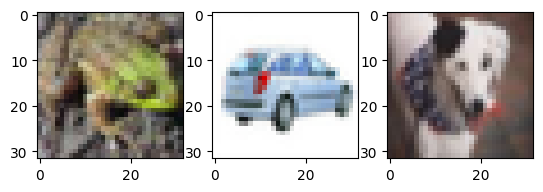
\includegraphics[width=0.95\columnwidth]{cifar-example-images}
\caption{CIFAR images from the frog, car, and dog classes.}
\label{fig1}
\end{figure}

That original research studied models with large numbers of trainable parameters (though the ResNet architecture in
general requires many fewer parameters than standard CNN models to achieve good performance).
The smallest network in the original ResNet paper, ResNet-18, has 11.7 million parameters, according to torch-summary
analysis of the PyTorch ResNet implementation.

This research focuses on designing, training, and evaluating a model with ResNet architecture that has under five
million parameters, aiming to achieve high accuracy on CIFAR-10.
Using model definition and training code adapted from a reference implementation~\cite{kl:2021}, model
hyperparameters and training strategies are determined through experimentation on a validation set.
The final model produced from this process achieves accuracy of TBD on the CIFAR-10 test dataset.

\section{Methodology}

To design the optimal model for the task, a series of experiments is performed to determine the best architecture,
hyperparameters, and training strategies such as regularization, learning rate scheduling, and data augmentation.
The CIFAR-10 training dataset is split into 90\% for training and 10\% for validation.
Alternatives are evaluated based on quantitative metrics such as validation accuracy as well as qualitative assessment
of loss curve trends.

\subsection{Architecture}

Our model definition code implements the core ResNet feature of convolutional layers with skip connections as a
pipeline of block sequences, where a block contains two convolutional layers, each with batch normalization, plus the
skip connection.
The number of block sequences in the pipeline and the lengths of the individual block sequences form a descriptor of a
given model architecture.
For example, the ResNet-18 model has four block sequences, each of length 2, and can be identified by the architecture
descriptor 2-2-2-2.

The original ResNet research prefers sequences of at least two blocks.
Architectures with four such block sequences have more than 5 million trainable parameters, thus candidate
architectures for our task must contain at most three sequences.
Based on these constraints, the following architectures are candidates for evaluation: 2-2-2, 2-4-2, 2-5-2, 2-5-3,
and 3-5-3.
Because the upstream codebase explicitly required a pipeline of four block sequences, it was adapted to support an
arbitrary number of block sequences.

For these initial experiments, hyperparameters and other training details are drawn from the original ResNet paper and
the upstream repository defaults.
The learning rate is set to 0.1 and models are trained for 40 epochs with Stochastic Gradient Descent (SGD) at a batch
size of 128.
Early experimentation showed that at higher epochs, validation accuracy can stagnate while training accuracy continues
to improve.
As this is an indication of overfitting, these experiments implement early stopping of training when
training accuracy reaches between 97.0\% and 99.5\%, depending on the experiment.

\begin{figure*}[t]
\centering
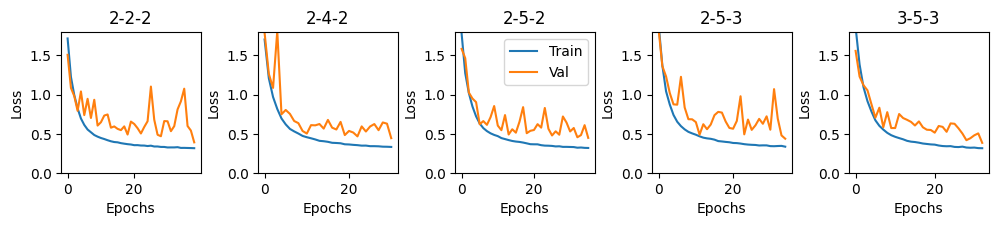
\includegraphics[width=0.99\textwidth]{loss-curves-5} % Reduce the figure size so that it is slightly narrower than the column.
\caption{Training and validation loss by architecture with constant learning rate}
\label{fig2}
\end{figure*}

\begin{table}[t]
\centering
%\resizebox{.95\columnwidth}{!}{
\begin{tabular}{|l|l|}
    \firsthline
    Arch & Val Acc    \\
    \hline
    2-2-2 & 86.56\%    \\
    2-4-2 & 84.74\%    \\
    2-5-2 & 84.98\%    \\
    2-5-3 & 85.32\%    \\
    3-5-3 & 87.00\%    \\
    \lasthline
\end{tabular}
%}
\caption{Validation accuracy by architecture with constant learning rate}
\label{table1}
\end{table}

The results of the initial architecure experiment are shown in Figure~\ref{fig2} and Table~\ref{table1}.
The most stable validation loss behavior is observed in architectures 2-4-2 and 3-5-3, but 2-2-2 and 3-5-3
have the greatest validation accuracy.
Before selecting a single architecture, we will consider learning rate scheduling to compare performance
with more stable loss trends.

\subsection{Training Strategies}

\subsubsection{Learning Rate Scheduling}

The initial architecture experiments were conducted with a constant learning rate of 0.1.
Other approaches under consideration are: step scheduling, as used by the original ResNet paper;
cosine annealing, as implemented in the upstream codebase; and adaptive scheduling that reduces the learning rate
when validation loss plateaus.
For these experiments, training is stopped early if the training accuracy reaches 97.5\%.

\begin{table}[b]
\centering
%\resizebox{.95\columnwidth}{!}{
\begin{tabular}{|l|r|}
    \firsthline
    Arch/LRS & Val Acc \%    \\
    \hline
    2-2-2 Step & 86.7    \\
    3-5-3 Step & 87.3    \\
    2-2-2 Cosine annealing & 92.1    \\
    3-5-3 Cosine annealing & 92.0    \\
    2-2-2 Adaptive-plateau & 92.2    \\
    3-5-3 Adaptive-plateau & 91.7    \\
    \lasthline
\end{tabular}
%}
\caption{Validation accuracy by architecture and Learning Rate Scheduler}
\label{table2}
\end{table}

\begin{figure}[b]
\centering
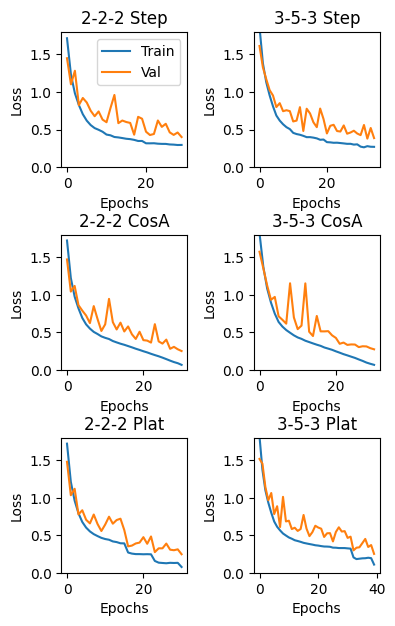
\includegraphics[width=0.98\columnwidth]{experiment-lrschedule-3x2}
\caption{Training and validation loss by architecture and learning rate scheduler.}
\label{fig3}
\end{figure}


The results of the learning rate scheduler experiment, shown in Table~\ref{table2} and Figure~\ref{fig3}, indicate that
the cosine annealing and adaptive-plateau schedulers outperform the step scheduler under the current
parameterization.
The cosine annealing scheduler shows a strong downward trend in training loss while validation loss
stays stagnant.
This suggests that the cosine annealing scheduler is prone to overfitting, so the
adaptive-plateau scheduler will be selected by default for subsequent experiments.
The validation accuracy of the 2-2-2 and 3-5-3 architectures is about the same,
and we elect to use the 3-5-3 architecture (4.9 million parameters) for its expressiveness
advantage, keeping in mind that the increased expressiveness means we must be vigilant
with respect to overfit.


\subsubsection{Optimizer}

The optimizer algorithm plays a key role in training, and Adam was considered as an alternative to the default SGD\@.
However, initial results showed Adam to be ineffective at the (somewhat large) learning rate $ 0.1 $.
Validation loss is extremely volatile
at that learning rate and training loss fails to converge.
Using learning rate $ 0.01 $, there is some improvement, but the model still fails to achieve more than 60\% validation
accuracy, even when trained to twice as many epochs as a model trained with SGD. More investigation is needed to
determine whether our implementation was flawed, more hyperparameter tuning is required, or
the algorithm is not well-suited to this type of model and/or dataset characteristics.

\subsubsection{Regularization}

A suboptimal trend observed in the experiments above is the training loss continuing to decrease in later
epochs while the validation accuracy stagnates.
A possible explanation of this phenomenon is that the gradient reaches a local minimum, and further training
refines the model within that local neighborhood and improvements are generalized.
Subsequent minor increases in validation accuracy at that point are likely the result of random fluctuations as the
model becomes overfitted to the training data.

To reduce overfitting, several strategies for regularization are considered:
introducing dropout into training, varying training data by augmentation, and increasing weight decay.
To test the effect of dropout, multiple dropout ``layers'' are inserted into the model at the input layer, before and
after the block sequence pipeline, and between each sequence in the block sequence pipeline.
Two dropout strategies are evaluated; in both cases, the input layer dropout rate is 20\%, and dropout rates of 20\%
and 50\% for the hidden layers are evaluated.
To test the effect of weight decay, the upstream codebase's default value of $ 0.0005 $ is compared to values of
$ 0 $, $ 0.00275 $, and $ 0.005 $.

For the dropout experiment, models were trained up to 80 epochs, instead of the 40 epoch limit in above experiments,
to account for how dropout may delay convergence.
Early stopping was imposed at training accuracy of 97.5\%.
The validation accuracies under varying dropout configurations, displayed in Table~\ref{table3},
are not substantially different, and the configuration with no dropout achieves maximum validation accuracy.
The configuration in which the input layer dropout rate is 20\% but hidden layers have no dropout
is a close second, and it is worthy of consideration because the model may have learned a more robust
representation of the input, but there is not enough evidence to deviate from the default zero-dropout
configuration.

\begin{table}[b]
\centering
%\resizebox{.95\columnwidth}{!}{
\begin{tabular}{|l|l|l|}
    \firsthline
    Input \% & Hidden \% & Val Acc \%    \\
    \hline
    0 & 0 & 91.8    \\
    20 & 0 & 91.4    \\
    20 & 20 & 91.2    \\
    20 & 50 & 89.7    \\
    \lasthline
\end{tabular}
%}
\caption{Validation accuracy under varying dropout rates. The input layer and hidden layer dropout rates are varied between 0 and 50\%.}
\label{table3}
\end{table}

INSERT weight decay experiment results


Additional data augmentation for the purpose of regularization is potentially worth investigating; the current
implementation includes random horizontal flip and random crop with 4 pixels of padding.

\subsection{Hyperparameters}

The 2-2-2 architecture selected from the above analysis was evaluated with three different values for the convolution
kernel size within each block.
The impact of other hyperparameters, such as the number of channels within blocks and the pool size in the average pool
layer, may be worthy of consideration, but their values were fixed at the upstream defaults to reduce the search space
for this investigation.
Experiments were conducted with models trained with convolution kernel sizes of 3 (the default), 5, and 7, and the
results are shown below.

INSERT convolution kernel size experiment results

Kernel size 3 is selected as the optimal kernel size because it achieve the highest validation accuracy.
The effect of varying the kernel size is not large, possibly because the CIFAR image size is quite small (32x32 pixels).

\section{Results}

The analysis above suggests that the best choice of architecture, training strategy, and hyperparameters is the 2-2-2
model with adaptive learning rate scheduler, weight decay 0.0005, 20\% input dropout and 50\% hidden dropout, and
convolution kernel size 3.
This model was trained to 100 epochs, with early stopping of training (at training accuracy 97.5\%) to avoid overfitting.
The checkpoint with the best validation accuracy was selected to be evaluated on the test data.
On the CIFAR-10 test dataset, which contains 10k images, the model's accuracy is TBD.

Most avenues of investigation ended with the choice to use parameters specified by the original ResNet researchers or
the upstream codebase, or to use near equivalents.
This suggests either that those authors had performed adequate tuning already or that further exploration of variables,
with more granular and systematic examination, is warranted.
Grid search with cross validation would be an appropriate technique for such exploration, given sufficient time and
computing resources.

\bibliography{aaai24}

\end{document}
